\documentclass[a4paper,12pt,openany,oneside]{article}
\usepackage[a4paper,top=2cm,bottom=2cm,left=2cm,right=3cm]{geometry}
\usepackage[utf8]{inputenc}
\usepackage{pgfplots}
\pgfplotsset{compat=1.12}
\usepgfplotslibrary{fillbetween}
\usetikzlibrary{patterns, quotes, angles}
\usepackage{amsmath}
\usepackage{animate}
\usepackage[hidelinks]{hyperref}

\title{Complex Numbers}
\author{Lorenzo Bonanni}
\date{October 2021}



\begin{document}
\maketitle
Sources:
\begin{itemize}
    \item \href{https://youtu.be/5PcpBw5Hbwo}{\color{blue}\textit{Complex number fundamentals | Lockdown math ep. 3}}
    \item \href{https://youtu.be/ZxYOEwM6Wbk}{\color{blue}\textit{What is Euler's formula actually saying? | Lockdown math ep. 4}}
\end{itemize}

\newpage
\section{Assumptions}
\begin{minipage}{.5\textwidth}
    \begin{itemize}
        \item There's a number i so that $i^2=-1$
        \item $i$ stays on a different number line that's perpendicular to Real Numbers
    \end{itemize}
\end{minipage}
\hspace{2cm}% NO SPACE!
\begin{minipage}{.2\textwidth}
    \begin{center}
        \begin{tikzpicture}[scale=0.6]
            \begin{scope}[thick,font=\scriptsize]
            % Axes:
            % Are simply drawn using line with the `->` option to make them arrows:
            % The main labels of the axes can be places using `node`s:
            \draw [->] (-3,0) -- (3,0);
            \draw [->] (0,-3) -- (0,3);
            
            \foreach \n in {-3,-2,-1,1,2,3}{
                \draw (\n,-2pt) -- (\n,2pt)   node [above] {$\n$};
                \draw (-2pt,\n) -- (2pt,\n)   node [right] {$\n i$};
            }
            \end{scope}
        \end{tikzpicture}
    \end{center}
\end{minipage}


\section{Operations}
\subsection{Sum}
\begin{minipage}{.4\textwidth}
    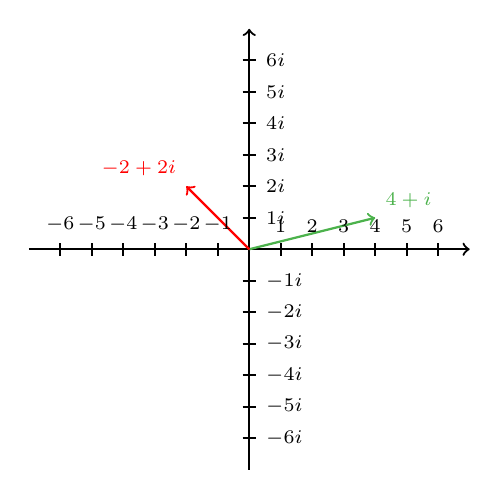
\begin{tikzpicture}[scale=0.40]
        \begin{scope}[thick,font=\scriptsize]
        % Axes:
        % Are simply drawn using line with the `->` option to make them arrows:
        % The main labels of the axes can be places using `node`s:
        \draw [->] (-7,0) -- (7,0);
        \draw [->] (0,-7) -- (0,7);
        \draw [->, color=green!40!gray] (0,0) -- (4, 1) node [above right] {$4+i$};
        \draw [->, color=red] (0,0) -- (-2, 2) node [above left] {$-2+2i$};
        
        \foreach \n in {-6,...,-1,1,2,...,6}{%
            \draw (\n,-6pt) -- (\n,6pt)   node [above] {$\n$};
            \draw (-6pt,\n) -- (6pt,\n)   node [right] {$\n i$};
        }
        \end{scope}
    \end{tikzpicture}
\end{minipage}
\hspace{1cm}% NO SPACE!
\begin{minipage}{.6\textwidth}
    To sum those two vectors $-2+2i$ and $4+i$ we simply divide the imaginary part from the real one and then we sum those single components.\\
    \textbf{Real Part:} $(4-2)$\\
    \textbf{Imaginary Part:} $(1-2)i$\\
    So the \textbf{result} is $2+3i$
\end{minipage}
\subsection{Multiplication}
Suppose we have the point (3,2) what is the 90° rotation of that point counterclockwise?\\
\\
\begin{center}
    \begin{minipage}{.25\textwidth}
        \begin{tikzpicture}[scale=0.40]
            \begin{scope}[thick,font=\scriptsize]
            % Axes:
            % Are simply drawn using line with the `->` option to make them arrows:
            % The main labels of the axes can be places using `node`s:
            \draw [->] (-7,0) -- (7,0);
            \draw [->] (0,-7) -- (0,7);
            % \draw [->, color=green!40!gray] (0,0) -- (4, 1) node [above right] {$4+i$};
            % \draw [->, color=red] (0,0) -- (-2, 2) node [above left] {$-2+2i$};
            \draw (3,2) node[anchor=south] {\textbullet};
            
            \foreach \n in {-6,...,-1,1,2,...,6}{%
                \draw (\n,-6pt) -- (\n,6pt)   node [above] {$\n$};
                \draw (-6pt,\n) -- (6pt,\n)   node [right] {$\n i$};
            }
            \end{scope}
        \end{tikzpicture}
    \end{minipage}
    \hspace{2cm}% NO SPACE!
    \begin{minipage}{.25\textwidth}
        To find out let's rotate the Entire plane 90°
    \end{minipage}
    \hspace{1cm}% NO SPACE!
    \begin{minipage}{.25\textwidth}
        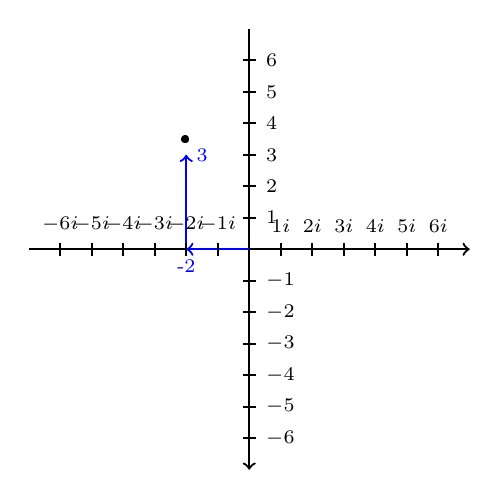
\begin{tikzpicture}[scale=0.40]
            \begin{scope}[thick,font=\scriptsize]
            % Axes:
            % Are simply drawn using line with the `->` option to make them arrows:
            % The main labels of the axes can be places using `node`s:
            \draw [->] (-7,0) -- (7,0);
            \draw [<-] (0,-7) -- (0,7);
            \draw [thick, ->, color=blue] (0,0) -- (-2, 0) node [below] {-2};
            \draw [thick, ->, color=blue] (-2, 0) -- (-2, 3) node [right] {3};;
            % \draw [->, color=red] (0,0) -- (-2, 2) node [above left] {$-2+2i$};
            \draw (-2, 3) node[anchor=south] {\textbullet};
            
            \foreach \n in {-6,...,-1,1,2,...,6}{%
                \draw (\n,-6pt) -- (\n,6pt)   node [above] {$\n i$};
                \draw (-6pt,\n) -- (6pt,\n)   node [right] {$\n$};
            }
            \end{scope}
        \end{tikzpicture}
    \end{minipage}
\end{center}


\begin{center}
    \begin{minipage}{.4\textwidth}
        (3,2)$\rightarrow$90°$\rightarrow$(-2,3)
        \\[0.2cm]
        (a,b)$\rightarrow$90°$\rightarrow$(-b,a)
        \\[0.2cm]
        (-b,a)$\rightarrow$90°$\rightarrow$(-a,-b)
    \end{minipage}
    \hspace{0.5cm}% NO SPACE!
    \begin{minipage}{.4\textwidth}
        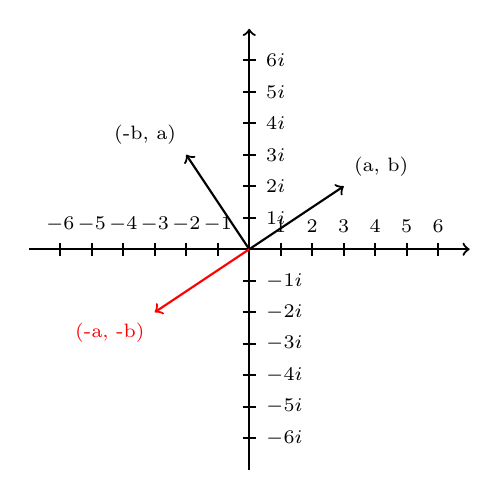
\begin{tikzpicture}[scale=0.40]
            \begin{scope}[thick,font=\scriptsize]
                % Axes:
                \draw [->] (-7,0) -- (7,0);
                \draw [->] (0,-7) -- (0,7);
                % ticks
                \foreach \n in {-6,...,-1,1,2,...,6}{
                    \draw (\n,-6pt) -- (\n,6pt)   node [above] {$\n$};
                    \draw (-6pt,\n) -- (6pt,\n)   node [right] {$\n i$};
                }
                
                % vectors
                \draw [->, color=black, thick] (0,0) -- (3, 2) node [above right] {(a, b)};
                \draw [->, color=black, thick] (0,0) -- (-2, 3) node [above left] {(-b, a)};
                \draw [->, color=red, thick] (0,0) -- (-3, -2) node [below left] {(-a, -b)};
            \end{scope}
        \end{tikzpicture}
    \end{minipage}
\end{center}

\noindent
Lets calculate the following equation $3*(3+2i)$:
\\[0.2cm]
$i*(3+2i) = 3i+2i^2 = 3i+2*(-1) = -2+3i$
\\[0.1cm]
As we can see the result is like rotating $3*(3+2i)$ by 90°

\subsubsection{3 Facts about Multiplications}
\begin{enumerate}
    \item $z*1=z$
    \item $z*i=Rot90(z)$
    \item $z*(c+di)=c*z+d*(zi)$
\end{enumerate}

\vspace{.5cm}
\noindent
Let's solve $(2+i)(2-i)$
\\[0.2cm]
$(2+i)(2-i) = 2*2+2i-2i-i^2 = 4+0i-(-1) = 5+0i = 5$

\vspace{1cm}
\noindent
\textbf{What is the complex number $z$ so that multiplying by $z$ has the effect of rotating 30°, or $\frac{\pi}{6}$ radians, counterclockwise?}
\\[0.3cm]
\begin{center}
    $z=cos(\pi/6)+isin(\pi/6)$\\[0.5cm]    
\end{center}

\begin{minipage}{.4\textwidth}
    \begin{tikzpicture}[scale=2.3,cap=round,>=latex]
        % draw the coordinates
        \draw[->] (-1.5cm,0cm) -- (1.5cm,0cm) node[right,fill=white] {$x$};
        \draw[->] (0cm,-1.5cm) -- (0cm,1.5cm) node[above,fill=white] {$y$};
    
        % draw the unit circle
        \draw (0cm,0cm) circle(1cm);
        
        % draw the horizontal and vertical coordinates
        % the placement is better this way
        \draw (-1.25cm,0cm) node[below=1pt] {$(-1,0)$}
              (1.25cm,0cm)  node[below=1pt] {$(1,0)$}
              (0cm,-1.25cm) node[fill=white] {$(0,-1)$}
              (0cm,1.25cm)  node[fill=white] {$(0,1)$};
        \draw [->, color=black, thick] (0,0) -- (0.95cm, 0.3cm) node [above left]
        {$z$};
        \draw [-, color=blue] (0,0) -- (1cm, 0cm) node [below left]{$cos(\frac{\pi}{6})$};
        \draw [-, color=green!50!gray, dotted, thick] (0.95cm,0) -- (0.95cm, 0.3cm) node [below right]{$sin(\frac{\pi}{6})$};
    \end{tikzpicture}
\end{minipage}
\hspace{2cm}
\begin{minipage}{.4\textwidth}
    From that we can derive that every angle $\alpha$ on a unit circle could be represented with a complex number as a rotation.\\ In the following way:
    \\[0.1cm]
    $\alpha=cos(\alpha)+isin(\alpha)$
\end{minipage}

\newpage
\begin{minipage}{.3\textwidth}
    $cis(\alpha)=1/cis(\alpha)$
    \\
    $1/cis(\alpha)=cis(-\alpha)$
\end{minipage}
\begin{minipage}{.2\textwidth}
    \begin{tikzpicture}[scale=2.3,cap=round,>=latex]
        % draw the coordinates
        \draw[->] (-1.5cm,0cm) -- (1.5cm,0cm) node[right,fill=white] {$x$};
        \draw[->] (0cm,-1.5cm) -- (0cm,1.5cm) node[above,fill=white] {$y$};
    
        % draw the unit circle
        \draw (0cm,0cm) circle(1cm);
        
        % draw the horizontal and vertical coordinates
        % the placement is better this way
        \draw (-1.25cm,0cm) node[above=1pt] {$(-1,0)$}
              (1.25cm,0cm)  node[above=1pt] {$(1,0)$}
              (0cm,-1.25cm) node[fill=white] {$(0,-1)$}
              (0cm,1.25cm)  node[fill=white] {$(0,1)$};
        
        \draw
            (0.95,0.3) coordinate (a) node[above right] {$cis(\alpha)$}
            -- (0,0) coordinate (o)
            -- (1,0) coordinate (c) 
            pic["$\alpha$", color=blue, draw=blue, -, angle eccentricity=1.5, angle radius=1cm]
            {angle=c--o--a};
        
        \draw
            (0.95,-0.3) coordinate (a) node[below right] {$cis(-\alpha)$}
            -- (0,0) coordinate (o)
            pic["$-\alpha$", color=blue, draw=blue, -, angle eccentricity=1.5, angle radius=1cm]
            {angle=a--o--c};
        
    \end{tikzpicture}
\end{minipage}

\vspace{1cm}
\noindent
\begin{center}
    Usally people don't use $cis$ notation insted they express it using exponentials:
    $cis(\alpha)=cos(\alpha)+isin(\alpha) =e^{i\alpha}$
\end{center}

\section{Eulers Formula}
\subsection{Exponential}
\begin{minipage}{.2\textwidth}
    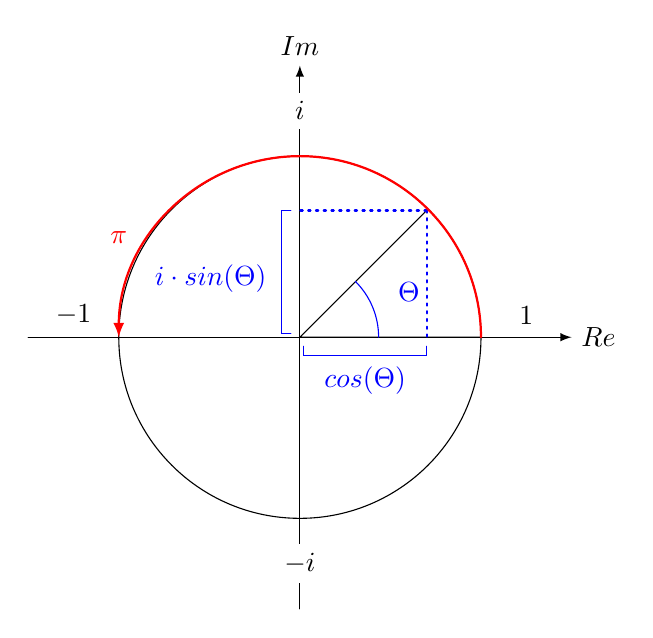
\begin{tikzpicture}[scale=2.3,cap=round,>=latex]
        % draw the coordinates
        \draw[->] (-1.5cm,0cm) -- (1.5cm,0cm) node[right,fill=white] {$Re$};
        \draw[->] (0cm,-1.5cm) -- (0cm,1.5cm) node[above,fill=white] {$Im$};
    
        % draw the unit circle
        \draw (0cm,0cm) circle(1cm);
        
        % draw the horizontal and vertical coordinates
        % the placement is better this way
        \draw (-1.25cm,0cm) node[above=1pt] {$-1$}
              (1.25cm,0cm)  node[above=1pt] {$1$}
              (0cm,-1.25cm) node[fill=white] {$-i$}
              (0cm,1.25cm)  node[fill=white] {$i$};
        
        \draw
            (0.7,0.7) coordinate (a)
            -- (0,0) coordinate (o)
            -- (1,0) coordinate (c) 
            pic["$\Theta$", color=blue, draw=blue, -, angle eccentricity=1.5, angle radius=1cm]
            {angle=c--o--a};
        
        \draw[dotted, thick, color=blue] (0.7,0.7) -- (0.7,0);
        
        \draw[dotted, thick, color=blue] (0.7,0.7) -- (0,0.7);
        
        \draw[color=blue]
            (-0.05, 0.7)
            -- (-0.1, 0.7) 
            -- (-0.1, 0.02) node[above=20pt, left=2pt] {$i\cdot sin(\Theta)$}
            -- (-0.05, 0.02);
            
        \draw[color=blue]
            (0.02, -0.05)
            -- (0.02, -0.1)
            -- (0.7, -0.1) node[below=9pt, left=4pt] {$ cos(\Theta)$}
            -- (0.7, -0.05);
            
        \draw[thick, ->, color=red] (1,0) arc[start angle=0, end angle=180,radius=1cm] node[above= 30pt] {$\pi$};
    \end{tikzpicture}
\end{minipage}
\hspace{5cm}% NO SPACE!
\begin{minipage}{.4\textwidth}
    $e \approx 2.71828...$
    \\
    $e^{i\Theta}=cos(\Theta)+isin(\Theta)$
    \\
    $e^{i\pi}=cos(\pi)+isin(\pi)=-1$
\end{minipage}
\\[0.2cm]
$e^x \neq e\cdot e...e$ ($e$ multiplied by its self $x$ times)
\\
$\downarrow$
\\
$\exp(x) = 1+x+\frac{x^2}{2}+\frac{x^3}{6}+\frac{x^4}{24}+...+\frac{x^n}{n!}+...$
\\[0.1cm]
$\exp(1) = 1+1+\frac{1}{2}+\frac{1}{6}+\frac{1}{24}+...+\frac{1}{n!}+...=2.71828...$ the series converges
\\[0.1cm]
$\exp(2) = 1+2+\frac{2^2}{2}+\frac{2^3}{6}+\frac{2^4}{24}+...+\frac{2^n}{n!}+..=7.389$
\\[0.3cm]
$\color{red}\exp(a+b) = \exp(a)\cdot \exp(b)$
\\[0.1cm]
$\exp(5) = \exp(1+1+1+1+1) = \exp(1)\cdot \exp(1)\cdot \exp(1) \cdot \exp(1) \cdot \exp(1)$ = $\exp(1)^5=e^5$
\\[0.1cm]
$\exp(\frac{1}{2})\cdot \frac{1}{2} = \exp(\frac{1}{2}+\frac{1}{2})=\exp(1)=e$
\\[0.1cm]
$\exp(-1)\cdot\exp(1)=\exp(0)=1$
\\[0.1cm]
$\exp(x)=e^x=\exp(1)^x$

\subsection{Powers of i}
\begin{minipage}{.2\textwidth}
    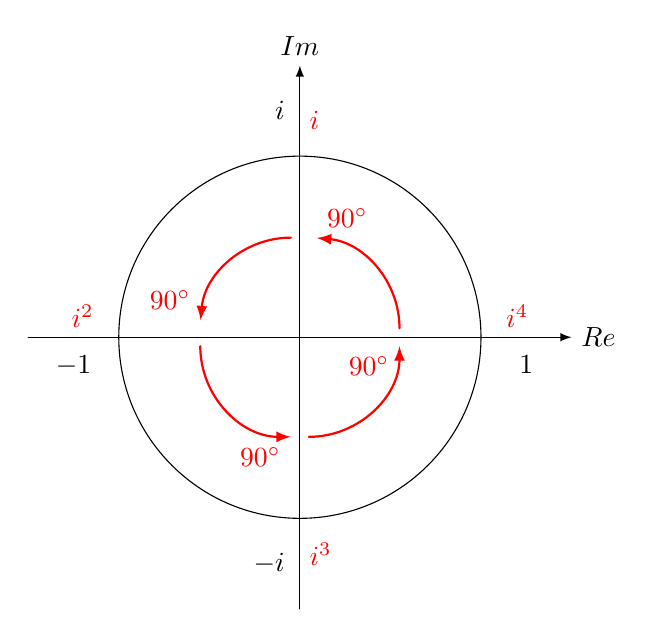
\begin{tikzpicture}[scale=2.3,cap=round,>=latex]
        % draw the coordinates
        \draw[->] (-1.5cm,0cm) -- (1.5cm,0cm) node[right,fill=white] {$Re$};
        \draw[->] (0cm,-1.5cm) -- (0cm,1.5cm) node[above,fill=white] {$Im$};
    
        % draw the unit circle
        \draw (0cm,0cm) circle(1cm);
        
        % draw the horizontal and vertical coordinates
        % the placement is better this way
        \draw (-1.25cm,0cm) node[below=3pt] {$-1$}
              (1.25cm,0cm)  node[below=3pt] {$1$}
              (0cm,-1.25cm) node[left=2pt] {$-i$}
              (0cm,1.25cm)  node[left=2pt] {$i$};
        
        \draw[thick, ->, color=red] (0.55,0.05) arc[start angle=0, end angle=85,radius=0.5cm] node[above right] {$90^{\circ}$};
        
        \draw[thick, ->, color=red] (-0.05,0.55) arc[start angle=90, end angle=175,radius=0.5cm] node[above left] {$90^{\circ}$};
        
        \draw[thick, ->, color=red] (-0.55,-0.05) arc[start angle=180, end angle=270,radius=0.5cm] node[below left] {$90^{\circ}$};
        
        \draw[thick, ->, color=red] (0.05,-0.55) arc[start angle=270, end angle=360,radius=0.5cm] node[below left] {$90^{\circ}$};
        
        \node at (1.2,0) [above, color=red]{$i^4$};
        \node at (-1.2,0) [above, color=red]{$i^2$};
        \node at (0,-1.2) [below,right, color=red]{$i^3$};
        \node at (0,1.2) [above,right, color=red]{$i$};
    \end{tikzpicture}
\end{minipage}
\hspace{6cm}
\begin{minipage}{.4\textwidth}
    $i^{-1}=\frac{1}{i}=i^3$
\end{minipage}

\subsection{What is the Claim of Euler's formula?}

\vspace{0.1cm}
$\exp(i\theta) = 1+i\theta+\frac{(i\theta)^2}{2}+\frac{(i\theta)^3}{6}+\frac{(i\theta)^4}{24}+...$
\\[0.2cm]
$\theta=1.0000$

    \begin{minipage}{.4\textwidth}
        \begin{tikzpicture}[scale=0.60]
            \begin{scope}[thick,font=\scriptsize]
                % Axes:
                \draw [->] (-5,0) -- (5,0);
                \draw [->] (0,-5) -- (0,5);
                % ticks
                \foreach \n in {-4,...,-1,1,2,...,4}{
                    \draw (\n,-4pt) -- (\n,4pt)  node [above, scale=0.6] {$\n$};
                    \draw (-4pt,\n) -- (4pt,\n)  node [right, scale=0.6] {$\n i$};
                }
                
                % vectors
                \draw [->, color=green!40!gray, thick] (0,0) -- (1, 0);
                \draw [->, color=yellow!60!gray, thick] (1,0) -- (1, 1);
                \draw [->, color=blue!50!gray, thick] (1,1) -- (0.5, 1);
                \draw [->, color=red!50!gray, thick] (0.5,1) -- (0.5, 0.84);
                \draw [->, color=orange!50!gray, thick] (0.5, 0.84) -- (0.5416, 0.84);
            \end{scope}
        \end{tikzpicture}
    \end{minipage}
    \begin{minipage}{.4\textwidth}
        As we can see Euler's formula is simply a sum of vectors but if we add a unit circle we'll see something special
    \end{minipage}
    
    \begin{minipage}{.4\textwidth}
        The Exponential always sits on the unit circle, as such we can interpret $e^{i\theta}$ as a movement on the unit circle
    \end{minipage}
    \hspace{2cm}
    \begin{minipage}{.4\textwidth}
        \begin{tikzpicture}[scale=1.5]
            \begin{scope}[thick,font=\scriptsize]
                % Axes:
                \draw [->] (-2,0) -- (2,0);
                \draw [->] (0,-2) -- (0,2);
                
                % ticks
                \draw (-1.25cm,0cm) node[below=2pt, scale=0.6] {$-1$}
                (1.25cm,0cm)  node[below=2pt, scale=0.6] {$1$}
                (0cm,-1.25cm) node[right=2pt,scale=0.6] {$-i$}
                (0cm,1.25cm)  node[right=2pt, scale=0.6] {$i$};
                
                % draw the unit circle
                \draw (0cm,0cm) circle(1cm);
                
                \def\itetha{(0, 1)};
                
                % vectors
                \draw [->, color=green!40!gray, thick] (0,0) -- (1, 0);
                \draw [->, color=yellow!60!gray, thick] (1,0) -- (1, 1);
                \draw [->, color=blue!50!gray, thick] (1,1) -- (0.5, 1);
                \draw [->, color=red!50!gray, thick] (0.5,1) -- (0.5, 0.84);
                \draw [->, color=orange!50!gray, thick] (0.5, 0.84) -- (0.5416, 0.84);
            \end{scope}
        \end{tikzpicture}
    \end{minipage}
    
    
    \newpage
    \noindent
    This Particular Formula has a Particularity that independently from the value of $\theta$ the sum of vectors will always end up onto the unit circle
    \\[0.5cm]
    \begin{center}
        \begin{minipage}{.4\textwidth}
            \begin{center}
                $\theta = 1.5$
            \end{center}
            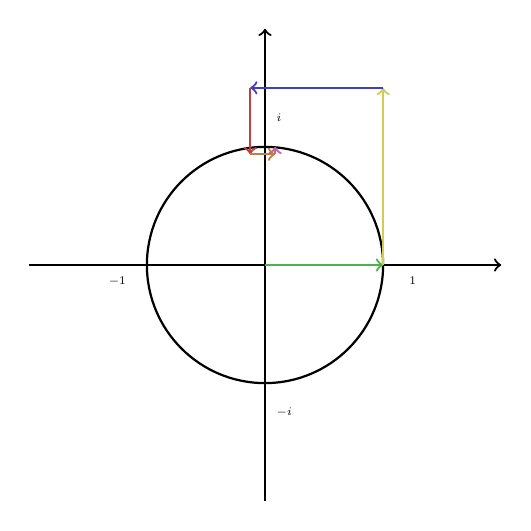
\begin{tikzpicture}[scale=1.5]
                \begin{scope}[thick,font=\scriptsize]
                    % Axes:
                    \draw [->] (-2,0) -- (2,0);
                    \draw [->] (0,-2) -- (0,2);
                    
                    % ticks
                    \draw (-1.25cm,0cm) node[below=2pt, scale=0.6] {$-1$}
                    (1.25cm,0cm)  node[below=2pt, scale=0.6] {$1$}
                    (0cm,-1.25cm) node[right=2pt,scale=0.6] {$-i$}
                    (0cm,1.25cm)  node[right=2pt, scale=0.6] {$i$};
                    
                    % draw the unit circle
                    \draw (0cm,0cm) circle(1cm);
                    
                    \def\itetha{(0, 1)};
                    
                    % vectors
                    \draw [->, color=green!40!gray, thick] (0,0) -- (1, 0);
                    \draw [->, color=yellow!60!gray, thick] (1,0) -- (1, 1.5);
                    \draw [->, color=blue!50!gray, thick] (1,1.5) -- (-0.125, 1.5);
                    \draw [->, color=red!50!gray, thick] (-0.125, 1.5) -- (-0.125, 0.9375);
                    \draw [->, color=orange!50!gray, thick] (-0.125, 0.9375) -- (0.0859375, 0.9375);
                    \draw [->, color=magenta!50!gray, thick] (0.0859375, 0.9375) -- (0.0859375, 1.00078125);
                \end{scope}
            \end{tikzpicture}
        \end{minipage}
        \begin{minipage}{.4\textwidth}
            \begin{center}
                $\theta = 2.2$
            \end{center}
            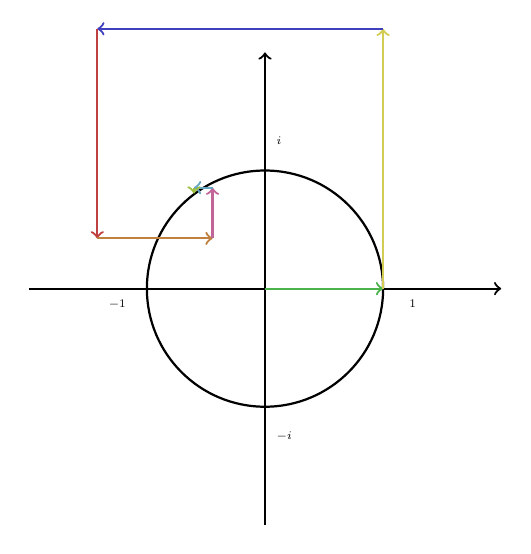
\begin{tikzpicture}[scale=1.5]
                \begin{scope}[thick,font=\scriptsize]
                    % Axes:
                    \draw [->] (-2,0) -- (2,0);
                    \draw [->] (0,-2) -- (0,2);
                    
                    % ticks
                    \draw (-1.25cm,0cm) node[below=2pt, scale=0.6] {$-1$}
                    (1.25cm,0cm)  node[below=2pt, scale=0.6] {$1$}
                    (0cm,-1.25cm) node[right=2pt,scale=0.6] {$-i$}
                    (0cm,1.25cm)  node[right=2pt, scale=0.6] {$i$};
                    
                    % draw the unit circle
                    \draw (0cm,0cm) circle(1cm);
                    
                    \def\itetha{(0, 1)};
                    
                    % vectors
                    \draw [->, color=green!40!gray, thick] (0,0) -- (1, 0);
                    \draw [->, color=yellow!60!gray, thick] (1,0) -- (1, 2.2);
                    \draw [->, color=blue!50!gray, thick] (1, 2.2) -- (-1.4200000000000004, 2.2);
                    \draw [->, color=red!50!gray, thick] (-1.4200000000000004, 2.2) -- (-1.4200000000000004, 0.4253333333333329);
                    \draw [->, color=orange!50!gray, thick] (-1.4200000000000004, 0.4253333333333329) -- (-0.4439333333333334, 0.4253333333333329);
                    \draw [->, color=magenta!50!gray, thick] (-0.4439333333333334, 0.4253333333333329) -- (-0.4439333333333334, 0.8548026666666664);
                    \draw [->, color=cyan!50!gray, thick] (-0.4439333333333334, 0.8548026666666664) -- (-0.6014054222222224, 0.8548026666666664);
                    \draw [->, color=lime!50!gray, thick] (-0.6014054222222224, 0.8548026666666664) -- (-0.6014054222222224, 0.8053114387301584);
                \end{scope}
            \end{tikzpicture}
        \end{minipage}
    \end{center}
    That means that plugin in a value of $\theta$ into the formula means walking $\theta$ units around the unit circle.
    
    \vspace{0.5cm}
    \noindent
    An interesting propriety of Euler's formula is that plugging in $\pi$ as the value of $\theta$ gives us -1.
    
    \vspace{0.5cm}
    \noindent
    To summarize the claim of Euler's Formula is that given:
    \begin{itemize}
        \item \textbf{real number} $\rightarrow$ $exp(x) = exp(1)^x = e^x$
        \item \textbf{immaginary number} $\rightarrow$ the function is periodic with a period of $2\pi$
    \end{itemize}
\end{document}
